\documentclass[11pt]{article}
\usepackage[T1]{fontenc}
\usepackage{lmodern}
\usepackage{microtype}
\usepackage{amsmath,amssymb,amsthm}
\usepackage{graphicx}
\usepackage{booktabs}
\usepackage{siunitx}
\usepackage{xcolor}
\usepackage{tikz}
\usetikzlibrary{positioning,arrows.meta,calc,shapes.geometric,decorations.pathmorphing,patterns}
\usepackage{pgfplots}
\pgfplotsset{compat=1.18}
\usepackage{hyperref}
\usepackage{cleveref}

\begin{document}
\section{Plots}
REVISION. A document with a pgfplots-heavy preamble and one plot.

\begin{figure}[h]
  \centering
  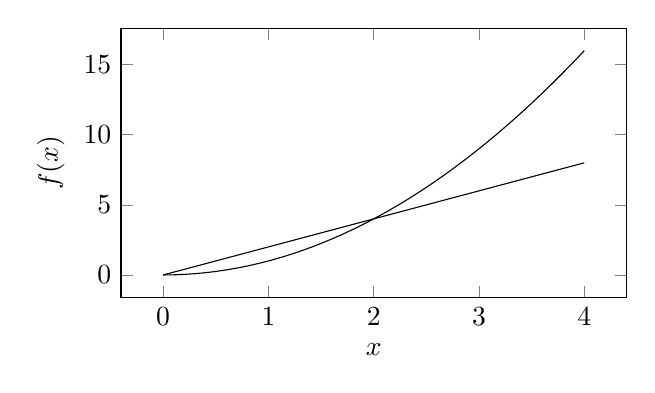
\begin{tikzpicture}
    \begin{axis}[width=8cm, height=5cm, xlabel={$x$}, ylabel={$f(x)$}]
      \addplot[domain=0:4, samples=40] {x^2};
      \addplot[domain=0:4, samples=40] {2*x};
    \end{axis}
  \end{tikzpicture}
  \caption{Two functions.}
\end{figure}
\end{document}
